\documentclass[11pt, oneside]{article}   	% use "amsart" instead of "article" for AMSLaTeX format
\usepackage{geometry}                		% See geometry.pdf to learn the layout options. There are lots.
\geometry{letterpaper}                   		% ... or a4paper or a5paper or ... 
%\geometry{landscape}                		% Activate for for rotated page geometry
%\usepackage[parfill]{parskip}    		% Activate to begin paragraphs with an empty line rather than an indent
\usepackage{graphicx}				% Use pdf, png, jpg, or eps§ with pdflatex; use eps in DVI mode
								% TeX will automatically convert eps --> pdf in pdflatex		
\usepackage{amssymb}
\usepackage{amsmath}
\usepackage{parskip}
\usepackage{color}

\title{Varberg and K1}
%\author{The Author}
%\section{}
% \subsection*{R code}
\date{}							% Activate to display a given date or no date

\graphicspath{{/Users/telliott_admin/Tex/png/}}

% \begin{center} 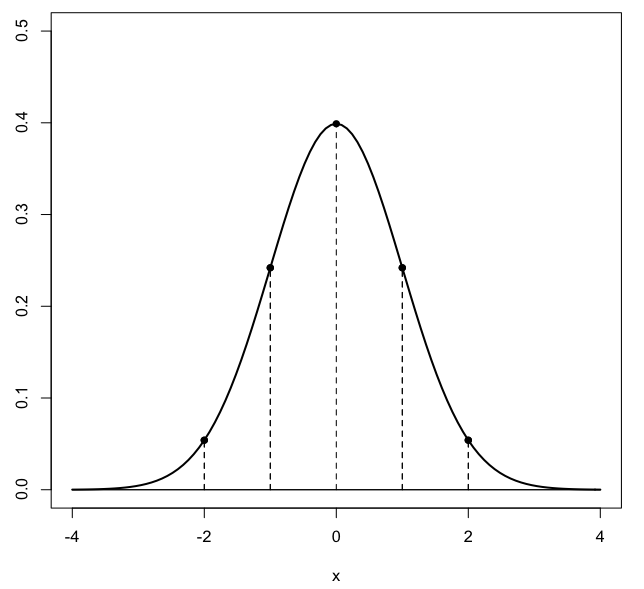
\includegraphics [scale=0.4] {gauss3.png} \end{center}

\begin{document}
\maketitle
\Large
\noindent
K2 says that orbits "sweep out equal areas in equal times".

Here we start from Newton's force directed toward the sun, the centripetal force, and we will show that the motion stays in a plane, that the orbits are (or can be) ellipses (K1), and also imply K2.

Again, this is Feynman's argument (and notation)
\[ \frac{d}{dt} ( \mathbf{r} \times \mathbf{v}) = \frac{d}{dt} ( \mathbf{r} \times \dot{\mathbf{r}}) = 0 \]
This is zero because you get two terms from the derivative of the cross-product:  one is $\dot{\mathbf{r}} \times \dot{\mathbf{r}} = 0$ , and the second one is $\mathbf{r} \times \ddot{\mathbf{r}}$, which is zero because these two vectors point in opposite directions by the centripetal force postulate.

Therefore,  $\mathbf{r} \times \dot{\mathbf{r}}$ is constant.  We will say that
\[ \mathbf{r} \times \dot{\mathbf{r}} = \mathbf{h} \]
\[ |\mathbf{h}| = h = 2 \ \frac{dA}{dt} \]
If $\mathbf{h} = 0$, there is no force, and just straight-line motion.  But for  $\mathbf{h} \ne 0$, then $\mathbf{r}$ and $\dot{\mathbf{r}}$ are in a plane that doesn't change with time, and $\mathbf{h}$ is the normal vector of that plane.
\[ h = | \mathbf{r} \times \dot{\mathbf{r}} | = |\mathbf{r} \times \frac{d\mathbf{r}}{dt} | \]

At this point, Varberg reverse the argument and show that planar motion and K2 imply a centripetal force.  But this is just Feynman's dots, which we already went through.

\subsection*{Kepler's First Law K1}
Now, we make an additional hypothesis due to Newton, which is that the acceleration is proportional to the inverse square of the distance from the sun (origin), and pointed toward it.
\[ \mathbf{a} = \ddot{\mathbf{r}} = - \frac{GM}{r^2} \mathbf{u_r} \]
where (as before) $\mathbf{u_r}$ is the unit vector in the $\mathbf{r}$ direction (i.e. equal to $\mathbf{r}/|\mathbf{r}|$), and $GM$ is a constant.

The first of three main steps in the proof is to take the cross-product with $\hat{\mathbf{k}}$ (as the text says, "this allows us to introduce the area information in vectorial form")
\[ \ddot{\mathbf{r}} \times \hat{\mathbf{k}} = - \frac{GM}{r^2} \ \mathbf{u_r} \times \hat{\mathbf{k}} = \frac{GM}{r^2} \ \mathbf{u_\theta} \]
(recall that we "go to the left" for $\mathbf{u_\theta}$).  

\[ \mathbf{u_r} \times \mathbf{u_{\theta}} = \hat{\mathbf{k}} \]
\[ \hat{\mathbf{k}} \times \mathbf{u_r} = \mathbf{u_{\theta}} \]
\[ \mathbf{u_{\theta}} \times \hat{\mathbf{k}} = \mathbf{u_r} \]

It should not be surprising that the cross-product brings us back to $\mathbf{u_\theta}$, since we aligned $\mathbf{u_r} \times \mathbf{u_{\theta}}$ with $\hat{\mathbf{k}}$, but note we're doing the product in reverse order, hence the minus sign.

From our discussion of the unit vectors and parametrization,
\[ \frac{d}{dt} \ \mathbf{u_r} = \dot{\mathbf{u}}_\mathbf{r} = \frac{d\theta}{dt} \ \mathbf{u_\theta} = \omega \mathbf{u_\theta} \]
\[ \mathbf{u_\theta} = \frac{\dot{\mathbf{u}}_{\mathbf{r}}}{\omega} \]
and from K2
\[ \frac{d \theta}{dt} = \omega = \frac{h}{r^2} \]
Hence
\[  \mathbf{u_\theta} =  \frac{\dot{\mathbf{u}}_{\mathbf{r}}}{\omega} = \frac{\dot{\mathbf{u}}_{\mathbf{r}}}{h/r^2} \]
So the cross-product which we had as
\[ \ddot{\mathbf{r}} \times \hat{\mathbf{k}} = \frac{GM}{r^2} \  \mathbf{u_\theta} \]
is equal to
\[ = \frac{GM}{r^2} \  \frac{\dot{\mathbf{u}}_{\mathbf{r}}}{h/r^2} \]
\[ = \frac{GM}{h} \ \dot{\mathbf{u}}_{\mathbf{r}}  \]
This is really the key step in our whole adventure. 

The second clever thing we do here is to integrate with respect to time
\[ \int \ddot{\mathbf{r}} \times \hat{\mathbf{k}} = \int \frac{GM}{h} \ \dot{\mathbf{u}}_{\mathbf{r}}  \]
(remember that $GM$, $h$ and $\hat{\mathbf{k}}$ are all constant)
\[ \dot{\mathbf{r}} \times \hat{\mathbf{k}} = \frac{GM}{h} \ ( \mathbf{u_r} + \mathbf{E}) \]
where $ \mathbf{E}$ is a constant (vector) of integration.

The third step is to form the dot product of both sides with $\mathbf{r}$
\[ \mathbf{r} \cdot ( \dot{\mathbf{r}} \times \hat{\mathbf{k}}) = \frac{GM}{h} \ \mathbf{r} \cdot ( \mathbf{u_r} + \mathbf{E}) \]
using a vector identity, the left-hand side is
\[ \mathbf{r} \cdot ( \dot{\mathbf{r}} \times \hat{\mathbf{k}}) = (\mathbf{r} \times \dot{\mathbf{r}}) \cdot \hat{\mathbf{k}} \]
but 
\[ \mathbf{r} \times \dot{\mathbf{r}} = \mathbf{h} =  h \ \hat{\mathbf{k}} \]
so we have
\[ h \ \hat{\mathbf{k}} \cdot \hat{\mathbf{k}} = h \]
Putting it all together
\[ \mathbf{r} \cdot (\ddot{\mathbf{r}} \times \hat{\mathbf{k}}) = h = \frac{GM}{h} \ \mathbf{r} \cdot ( \mathbf{u_r} + \mathbf{E}) \]
\[ \frac{h^2}{GM} =  \mathbf{r} \cdot ( \mathbf{u_r}+ \mathbf{E}) \]
Recall that $ \mathbf{u_r}$ is the unit vector in the same direction as $\mathbf{r}$ so that $\mathbf{r} \cdot  \mathbf{u_r} = r$.

We can take $\mathbf{E}$ to be in the direction of $\mathbf{r}$ at time-zero so $\mathbf{r} \cdot \mathbf{E}$ is equal to $r$ times $e$ times the cosine of the angle between them at some later time.  Since $\mathbf{E}$ is a constant vector of integration, its magnitude $e$ can be anything depending on the initial conditions.

We have then
\[ r(1 + e \cos \theta) = \frac{h^2}{GM} \]
These curves in polar coordinates are conic sections.  If $e < 1$ the curve is an ellipse.
\begin{center} 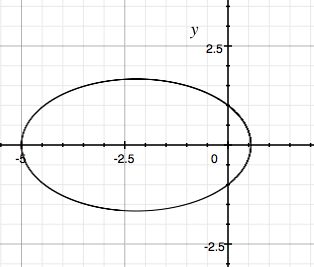
\includegraphics [scale=0.6] {quick_ellipse.png} \end{center}

The curve above is an ellipse with the formula
\[ r(1 + 0.8 \cos \theta) = 1 \]
$e$ is the eccentricity of the ellipse
\[ e^2 +  \frac{b^2}{a^2} = 1 \]
In the figure 
\[ e^2 = 0.8^2 = 0.64 \]
\[\frac{b^2}{a^2} = 1 - 0.64 = 0.36 \]
\[\frac{b}{a} = \sqrt{0.36} = 0.6 \]

\end{document}  